\section{Android - eine offene und mobile Plattform}
Android ist ein Betriebssystem, welches erstmals im November 2007 von Google, im Zuge der Ver\"offentlichung, des Android \ac{SDK} vorgestellt wurde. Das Betriebssystem bassiert auf dem Linux-Kernel und wird von der \ac{OHA} entwickelt. Es ist auf Ger\"aten wie Netbooks, Smartphones, Mobiltelefonen und Digitalkameras zu finden und Heute weit Verbreitet. \cite{Kuehn12}

\subsection{Android im Wandel der Zeiten}
\begin{wrapfigure}{r}{4,95cm}
\vspace{-13pt}
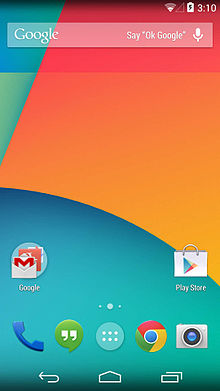
\includegraphics[width=4.95cm]{Bilder/Android4.jpg}
\caption{Android 4.4 Startbildschirm des Nexus 5 in Originalgr\"o\ss{}e \cite{WikiAndroid}}
\label{Der MongoDB-Chooser-Dialog}
\vspace{-20pt}
\end{wrapfigure}
Nach der Ver\"offentlichung des Android \ac{SDK} wurde 2008 mit dem "`G1"' das erste Smartphone mit dem neuen Betriebssystem Android vorgestellt. Ein direkten Vergleich zwischen Android und den von Apple stammenden iOS ging, zu dieser Zeit, klar zu Gunsten der Apple-Produkte aus.
% 
% Dem zu der Zeit noch Marktbeherschenden iOS und den iPhones, konnte 
 
Durch eine schnelle und konsequente Entwicklung konnten, der Firma Apple mit ihrem iOS, immer mehr Marktanteile abgenommen werden. Zum heutgen Zeitpunkt ist die Android-Plattform mit fast 85 Prozent Marktanteil im Bereich der Smartphonebetriebssysteme f\"uhrend. \cite{GolemMobileBetriebssystem}

Hardwarehersteller d\"urfen seit einiger Zeit nicht nur die Oberfl\"ache, sondern auch das Betriebssystem an sich auf ihre ganz speziellen Anforderungen anpassen, was zu einer gro\ss{}en Vielfalt der Plattform f\"uhrte. Ein pures unbearbeitetes Android ist zur Zeit nur auf Ger\"aten der "`Nexus-Reihe"' zu finden, welche zwar von verschiedenen Herstellern gebaut aber von Google vermarktet werden. Dies hat zur Folge das Systemupdates, auf Nexus-Ger\"aten, schneller und regelm\"a\ss{}iger zur Verf\"ugung stehen, da keine Anpassungen an den Updates, durch die Hardwarehersteller, vorgenommen werden m\"ussen.

Android ist momentan in der Version 4.4.4 alias "`Kit Kat"' auf dem Markt. Die Versionsnamen von Android sind immer nach einer S\"u\ss{}speise benannt und kommen in alphabetischer Reihenfolge auf den Markt. So folgte auf "`Jelly Bean"' die aktuelle Version Kit Kat. Eine nun schon in der Entwicklervorschau erschienene Version wird also mit "`L"' beginnen, weshalb diese Version momentan auch "`Android L"' genannt wird. Gut zu sehen ist, dass auf den Buchstaben J ein K folgte, welcher wiederum vom L abgel\"ost wird. \cite{WikiAndroid} \cite{Jung13}

Zus\"atzlich wurde dem Trend der "`Smartwatches"' folgend, im M\"arz 2014, ein speziell f\"ur Smartwatches angepasstes Android-System ver\"offentlicht, welches "`Android Wear"' hei\ss{}t. In dieser Arbeit wird jedoch nicht weiter auf Android Wear eingegangen, da dieses System nur im Zusammenspiel mit einem Smartphone in der Lage ist SMS zu empfangen. \cite{NextAndroidWear}

\subsection{Die Entwicklungsumgenung f\"ur Android}
Das schon angesprochene \ac{SDK} beinhaltet die folgenden Bestandteile:
\begin{itemize}
 \item Die eigentliche Entwicklungsumgenung mit Plugins
 \item Biblioteken und APIs
 \item Das Android Virtual Device
 \item Den USB-Treiber 
 \item Den SDK-Manager
 \item Das Programm dx
 
\end{itemize}

Nach dem downloaden und installieren der Android \ac{SDK} sind die eben genannten Bestandteile auf dem Rechner vorhanden und im Installationsverzeichnis zu finden. Die meisten Entwickler verwenden die \ac{IDE} Eclipse, f\"ur die eigentliche Programmierarbeit. Die im \ac{SDK} vorhandene Version von Eclipse enth\"alt das Plugin \ac{ADT}, welches viele Werkzeuge f\"ur die Android-Entwicklung mitbringt und welche sp\"ater genauer erl\"autert werden.

Eine andere Version des Android \ac{SDK} das sogenannte "`Android Studio"' bassiert auf der \ac{IDE} "`IntelliJ"'. Android Studio besitzt einige zus\"atzliche Features, wie die erweiterte "`Android Code-Completion"' oder die "`Multiple-APK generation"', welche es erlaubt eine Applikation gleichzeitig f\"ur Android und Android Wear zu erzeugen. Trotz der Vorteile, befindet sich das Android Studio noch in einer Beta-Phase und wird daher f\"ur die Entwicklung der App nicht verwendet. \cite{DevAndroidStudio}

Au\ss{}er der \ac{IDE} beinhaltet das Android \ac{SDK} die aktuellen Bibliotheken und APIs, welche f\"ur die Erstellung einer Applikation ben\"otigt werden. Dies beinhaltet auch Klassen, mit dessen Hilfe die zus\"atzliche Hardware in Android-Ger\"aten, wie das Notification-Light, angesprochen werden kann. Des weiteren ist auch eine lauff\"ahige Version des Androidbetriebssystems, welches f\"ur das Virtual Device ben\"otigt wird, vorhanden.

Das Virtual Device simuliert ein Smartphone am Rechner, auf dem die erstelle Applikation ausgef\"uhrt und getestet werden kann. Hierbei werden vom Virtual Device Debug-Information zur \ac{IDE} \"ubertragen, welche von dort aus angeschaut und ausgewertet werden k\"onnen.

Um eine geschriebene Applikation letztendlich nicht nur auf virtuellen Ger\"aten zu testen wird, unter Windows, ein USB-Treiber ben\"otigt. Dieser Treiber erm\"oglicht es, die Applikation auf ein reales Android-Ger\"at zu \"ubertragen und von dort aus zu Debuggen.
Um dies mit realer Hardware zu Testen, muss im entsprechenden Smartphone die "`Entwickler-Option"' aktiviert werden. Wie dies gemacht wird, wird im Kapitel ????? genauer beschrieben.

Der SDK-Manager ist ein Tool, mit dem die einzelnen Android-Version, Bibliotheken, APIs und Eclipse-Plugin-Versionen verwaltet und aktualisiert werden k\"onnen. Dies ist zum Beispiel hilfreich, wenn man eine Applikation unter verschiedenen Android-Version testen oder lauff\"ahig halten will.

Mit dem Namen dx wird ein Compiler bezeichnet, welcher Javaklassen unter Android lauff\"ahig macht. Mehr hierzu ist im folgenden Abschitt zu finden

\subsection{Dalvik anstelle der Java Virtual Machine}
Da eine Applikation f\"ur Android in Java geschrieben wird, liegt es nahe das auch hier eine virtuelle Maschine genutzt wird, welche ein Programm aus f\"uhrt. Im Android-System ist dies die \ac{DVM}, welche die Applikationen ausf\"uhrt.\cite{Android44}

\"Ahnlich wie die \emph{Java Virtual Machine} arbeitet auch Dalvik. Jedoch mit dem gro\ss{}en Unterschied, das Dalvik vom Google-Entwickler Dan Bornstein erdacht wurde um speziell auf leistungsschwachen mobilen Endger\"aten zu funktionieren.

Dalvik ist speziell daf\"ur entwickelt auf Prozessoren mit ARM-Architektur zu arbeiten, wobei die virtuelle Dalvik Maschine hier, im Gegensatz zur Java VM, in der Lage ist Hardwareregister direkt anzusprechen und zu nutzen. Durch die direkte Kommunikation mit der Hardware ergibt sich eine schnellere Verarbeitung des Codes als unter der Java VM direkt.

In der Theorie ist somit jede Javaklasse die unter Dalvik l\"auft auch unter der Java VM lauff\"ahig. Jedoch ergeben sich, in der Praxis, hier meist Schwierigkeiten durch Ein- und Ausgaben, da sich diese beim PC und Touchscreen grundlegend unterscheiden.

\subsubsection{Das Sandbox Prinzip}
Um Sicherheitsaspekten zu gen\"ugen besitzt Dalvik eine sogenannte Sandbox-Funktion, welche es erm\"oglicht Programme getrennt voneinander ausf\"uhren zu k\"onnen. F\"ur jedes auszuf\"uhrende Programm wird, unter Dalvik, eine neue Runtime-Umgegung erstellt, in der das Programm isoliert von anderen arbeitet. 
Dieses Prinzip wird Sandbox genannt, ja jedes Programm nur in seinem eigenen Sandkasten (Sandbox) "`spielen"' kann.

Dieses Vorgehen bringt sowohl Vorteile als auch Nachteile mit sich. Vorteilhaft ist, dass ein Programm nicht auf ein anderes zugreifen kann und dieses ungewollt ve\"andert, oder Daten aus einer anderen Programmausf\"uhrung abgreift. Gleichzeitig ist dieser Vorteil aber auch ein gro\ss{}er Nachteil, da ein gew\"unschter Austausch von Daten ebenfalls unterbunden wird.
Wie eine Daten\"ubertragen dennoch m\"oglich ist, wird im Kapitel ????? genauer behandelt.

\subsubsection{Von *.java zu *.dex}
Nachdem eine Javaklasse geschrieben wurde muss diese \"uber den Javacompiler (javac) in einen *.class-File umgewandelt werden. Dieser Class-File ist in der Theorie von jeder Java VM ausf\"uhrbar. Da die Klasse jedoch unter Dalvik optimiert laufen soll, muss sie ein weiteres mal Kompiliert werden. Diese zweite Kopilierungsstufe wird von dem schon erw\"ahnten Tool dx \"ubernommen. 
Der Dalvik-Compiler dx wandelt einen Class-File in einen von der \ac{DVM} ausf\"uhrbaren .dex-File um.

Dieser Zusammenhang ist in der Abbildung \ref{JavaZuDex} \"uber der Linie noch einmal zu sehen, da der beschriebene Zusammenhang auf dem Entwicklungsrecher passiert.

\begin{figure}[!ht]
\centering
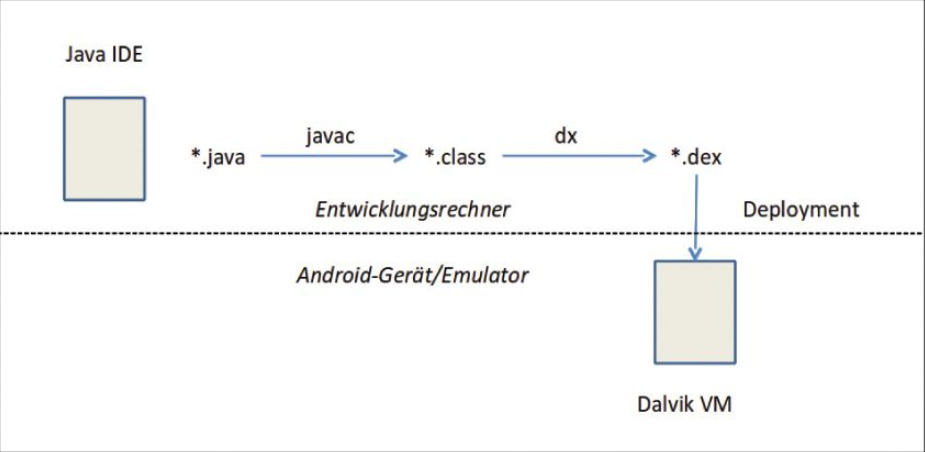
\includegraphics[width=12cm]{Bilder/JavaZuDex}
\caption{Von *.java zu *.dex \cite{Android44}}
\label{JavaZuDex}
\centering
\end{figure}